\section{Webサイトについて}\label{Webサイトについて}
娯楽ゲームの持つ教育的なメリットの周知を図り,印象を改善するためのWebサイトを作成した.

\subsection{概要}
WebサイトはHTMLとCSSを使用して作成し,ツールとしてBootstrapを用いた.

構成の詳細については以下の通りである.

\subsection{サイト構成}
Webサイトには図\ref{fig:サイト構成}のようにトップページにタグ一覧や教科一覧,ゲーム一覧のリンクを設置した.またアンケートの説明ページとGoogle Formsへのリンクを設置した.

トップページでは図\ref{fig:トップページ}に示すように説明文と各リンクへのボタンを設置した.
図内①には本研究の目的と対象者が閲覧した後に回答するアンケートへのリンクを,②には娯楽ゲームについての説明を表示し③に教育的メリットのタグ,教科,ゲーム一覧のページにリンクする各ボタンを設置した.
またページ左上部にメニューバーを設置し図\ref{fig:メニューバー}に示すようにどのページからも任意のページに遷移できるようにした.

\begin{figure}[H]
\begin{center}
 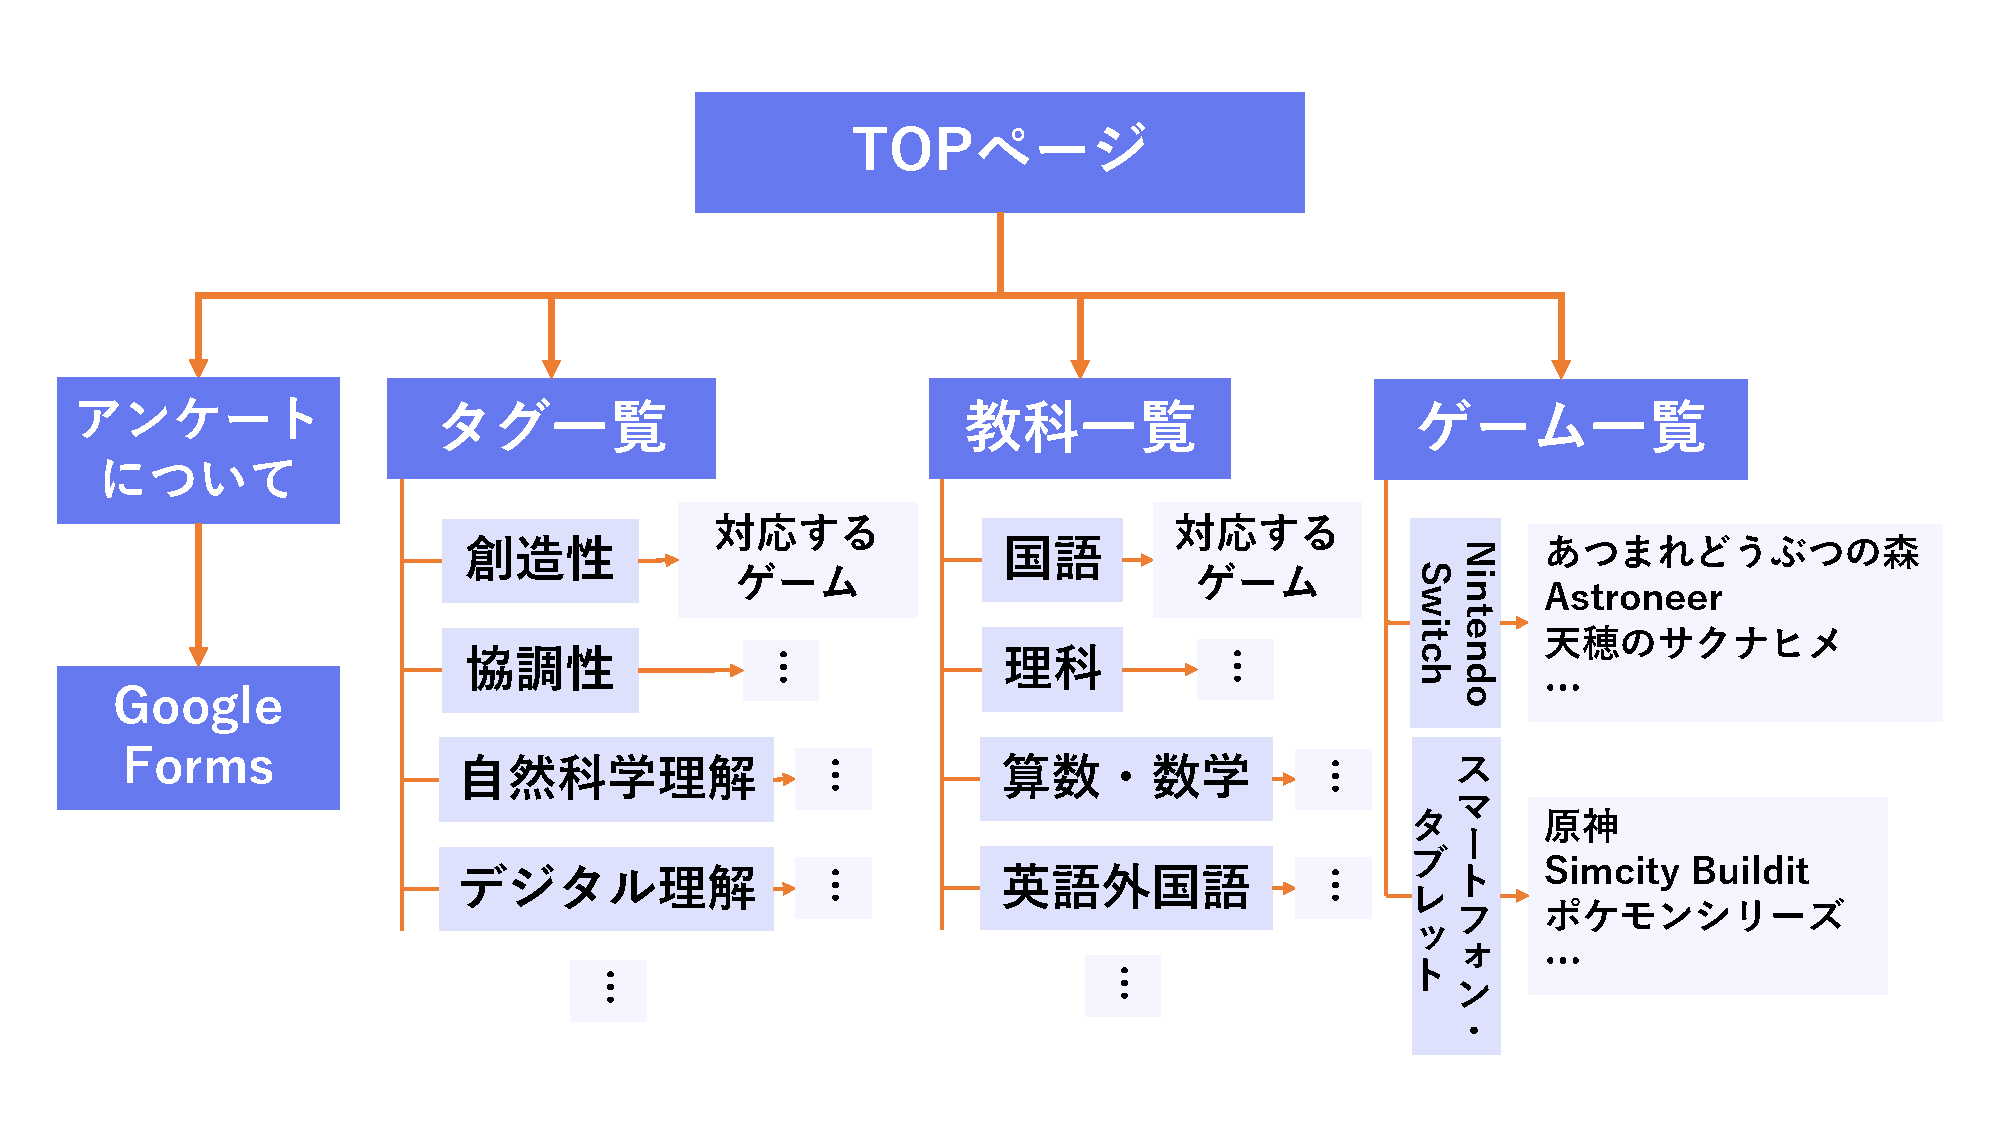
\includegraphics[keepaspectratio, scale=0.35]{PDF/サイト構成.pdf}
\end{center}
 \caption{サイト構成}
 \label{fig:サイト構成}
\end{figure}

\begin{figure}[H]
\begin{center}
 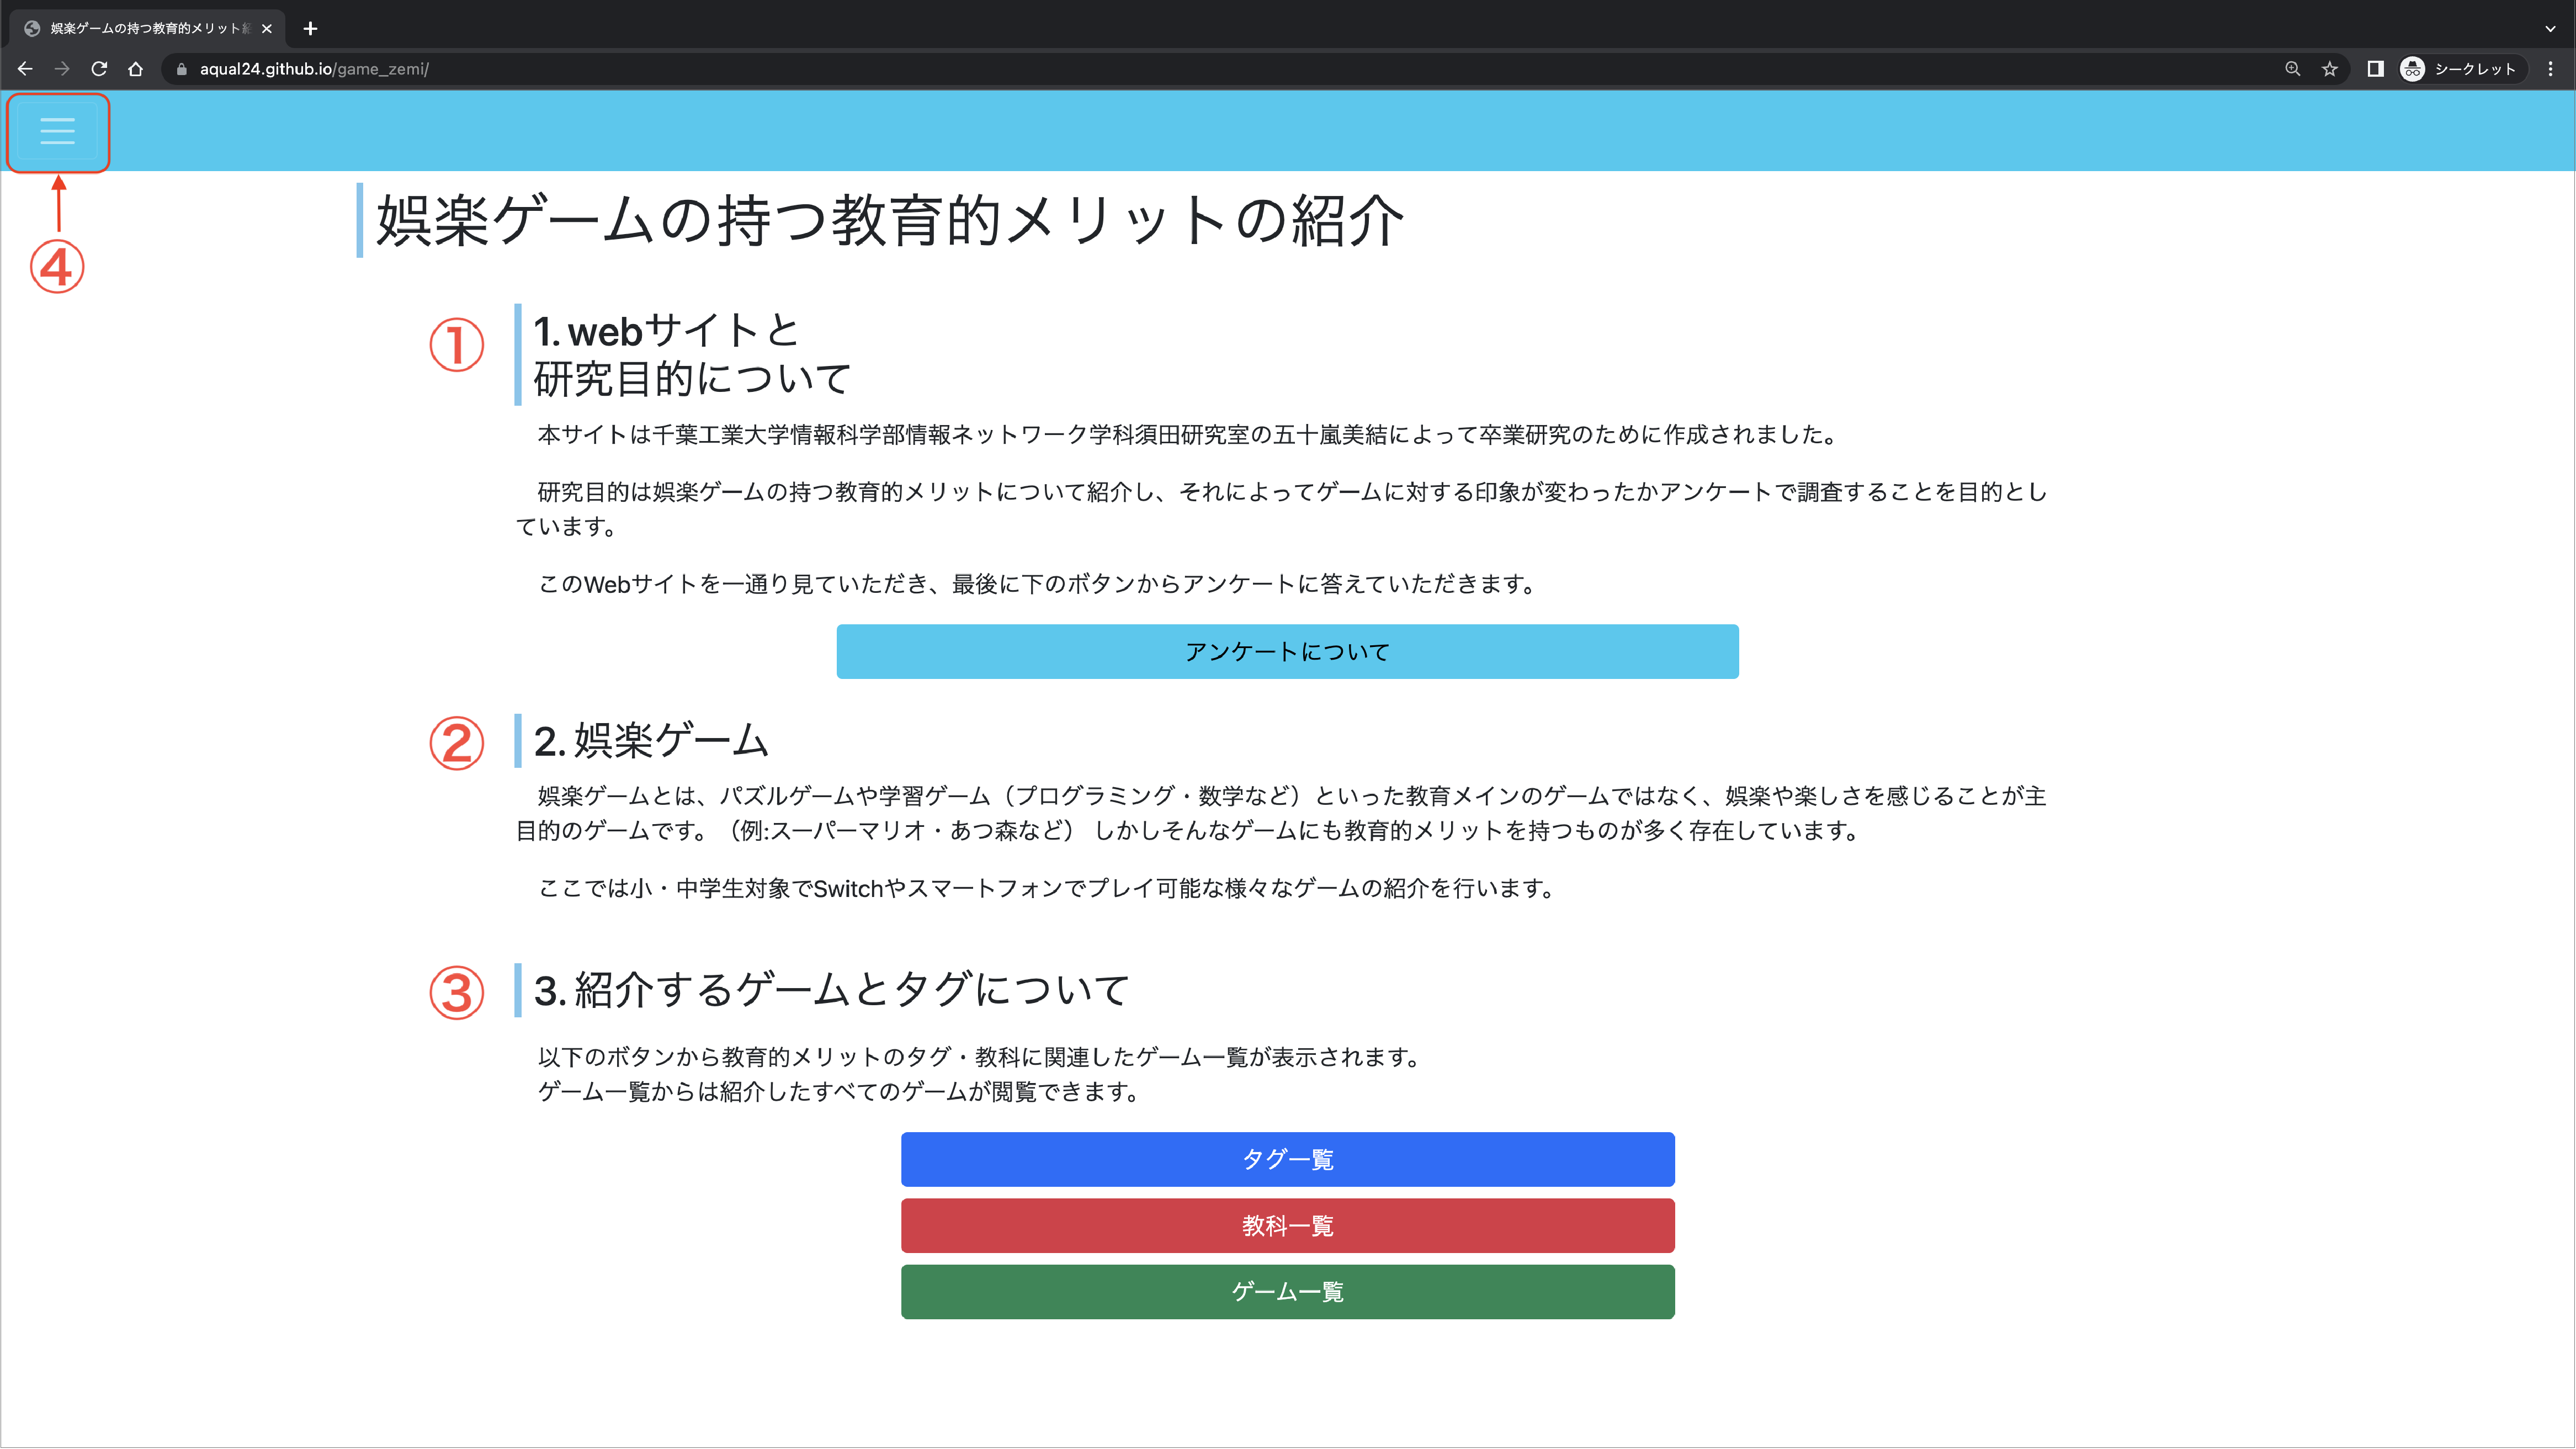
\includegraphics[keepaspectratio, scale=0.15]{PDF/toppage.pdf}
\end{center}
 \caption{トップページ}
 \label{fig:トップページ}
\end{figure}

\begin{figure}[H]
\begin{center}
 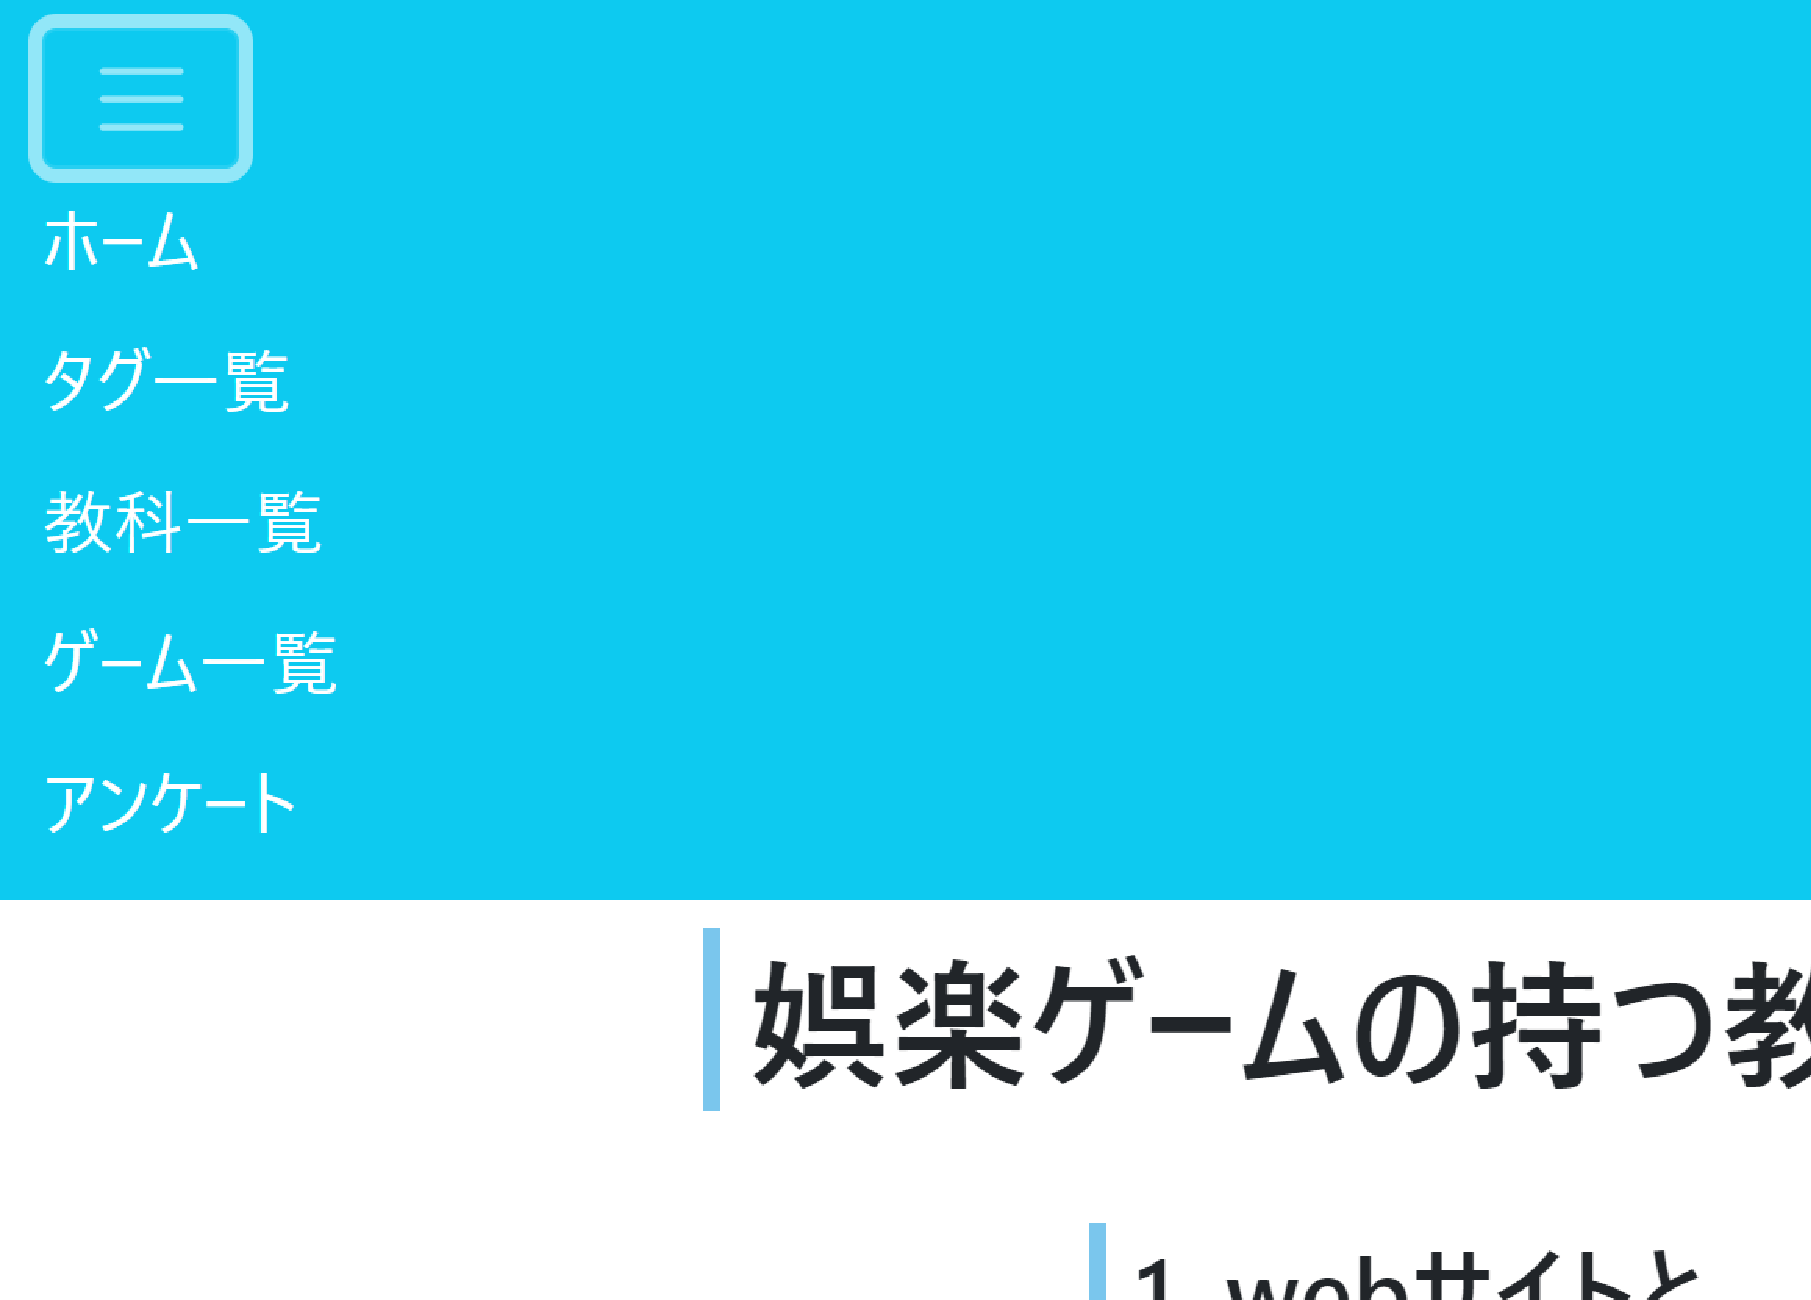
\includegraphics[keepaspectratio, scale=0.3]{PDF/menubar.pdf}
\end{center}
 \caption{メニューバー}
 \label{fig:メニューバー}
\end{figure}

タグ一覧のページでは図\ref{fig:タグページ}の⑤に示すように\ref{ゲームの種類}で解説する創造性や自然科学理解といった教育的なメリットを表示し,アコーディオンメニューで関連するゲームの記事へのリンクを設置した.

\begin{figure}[H]
\begin{center}
 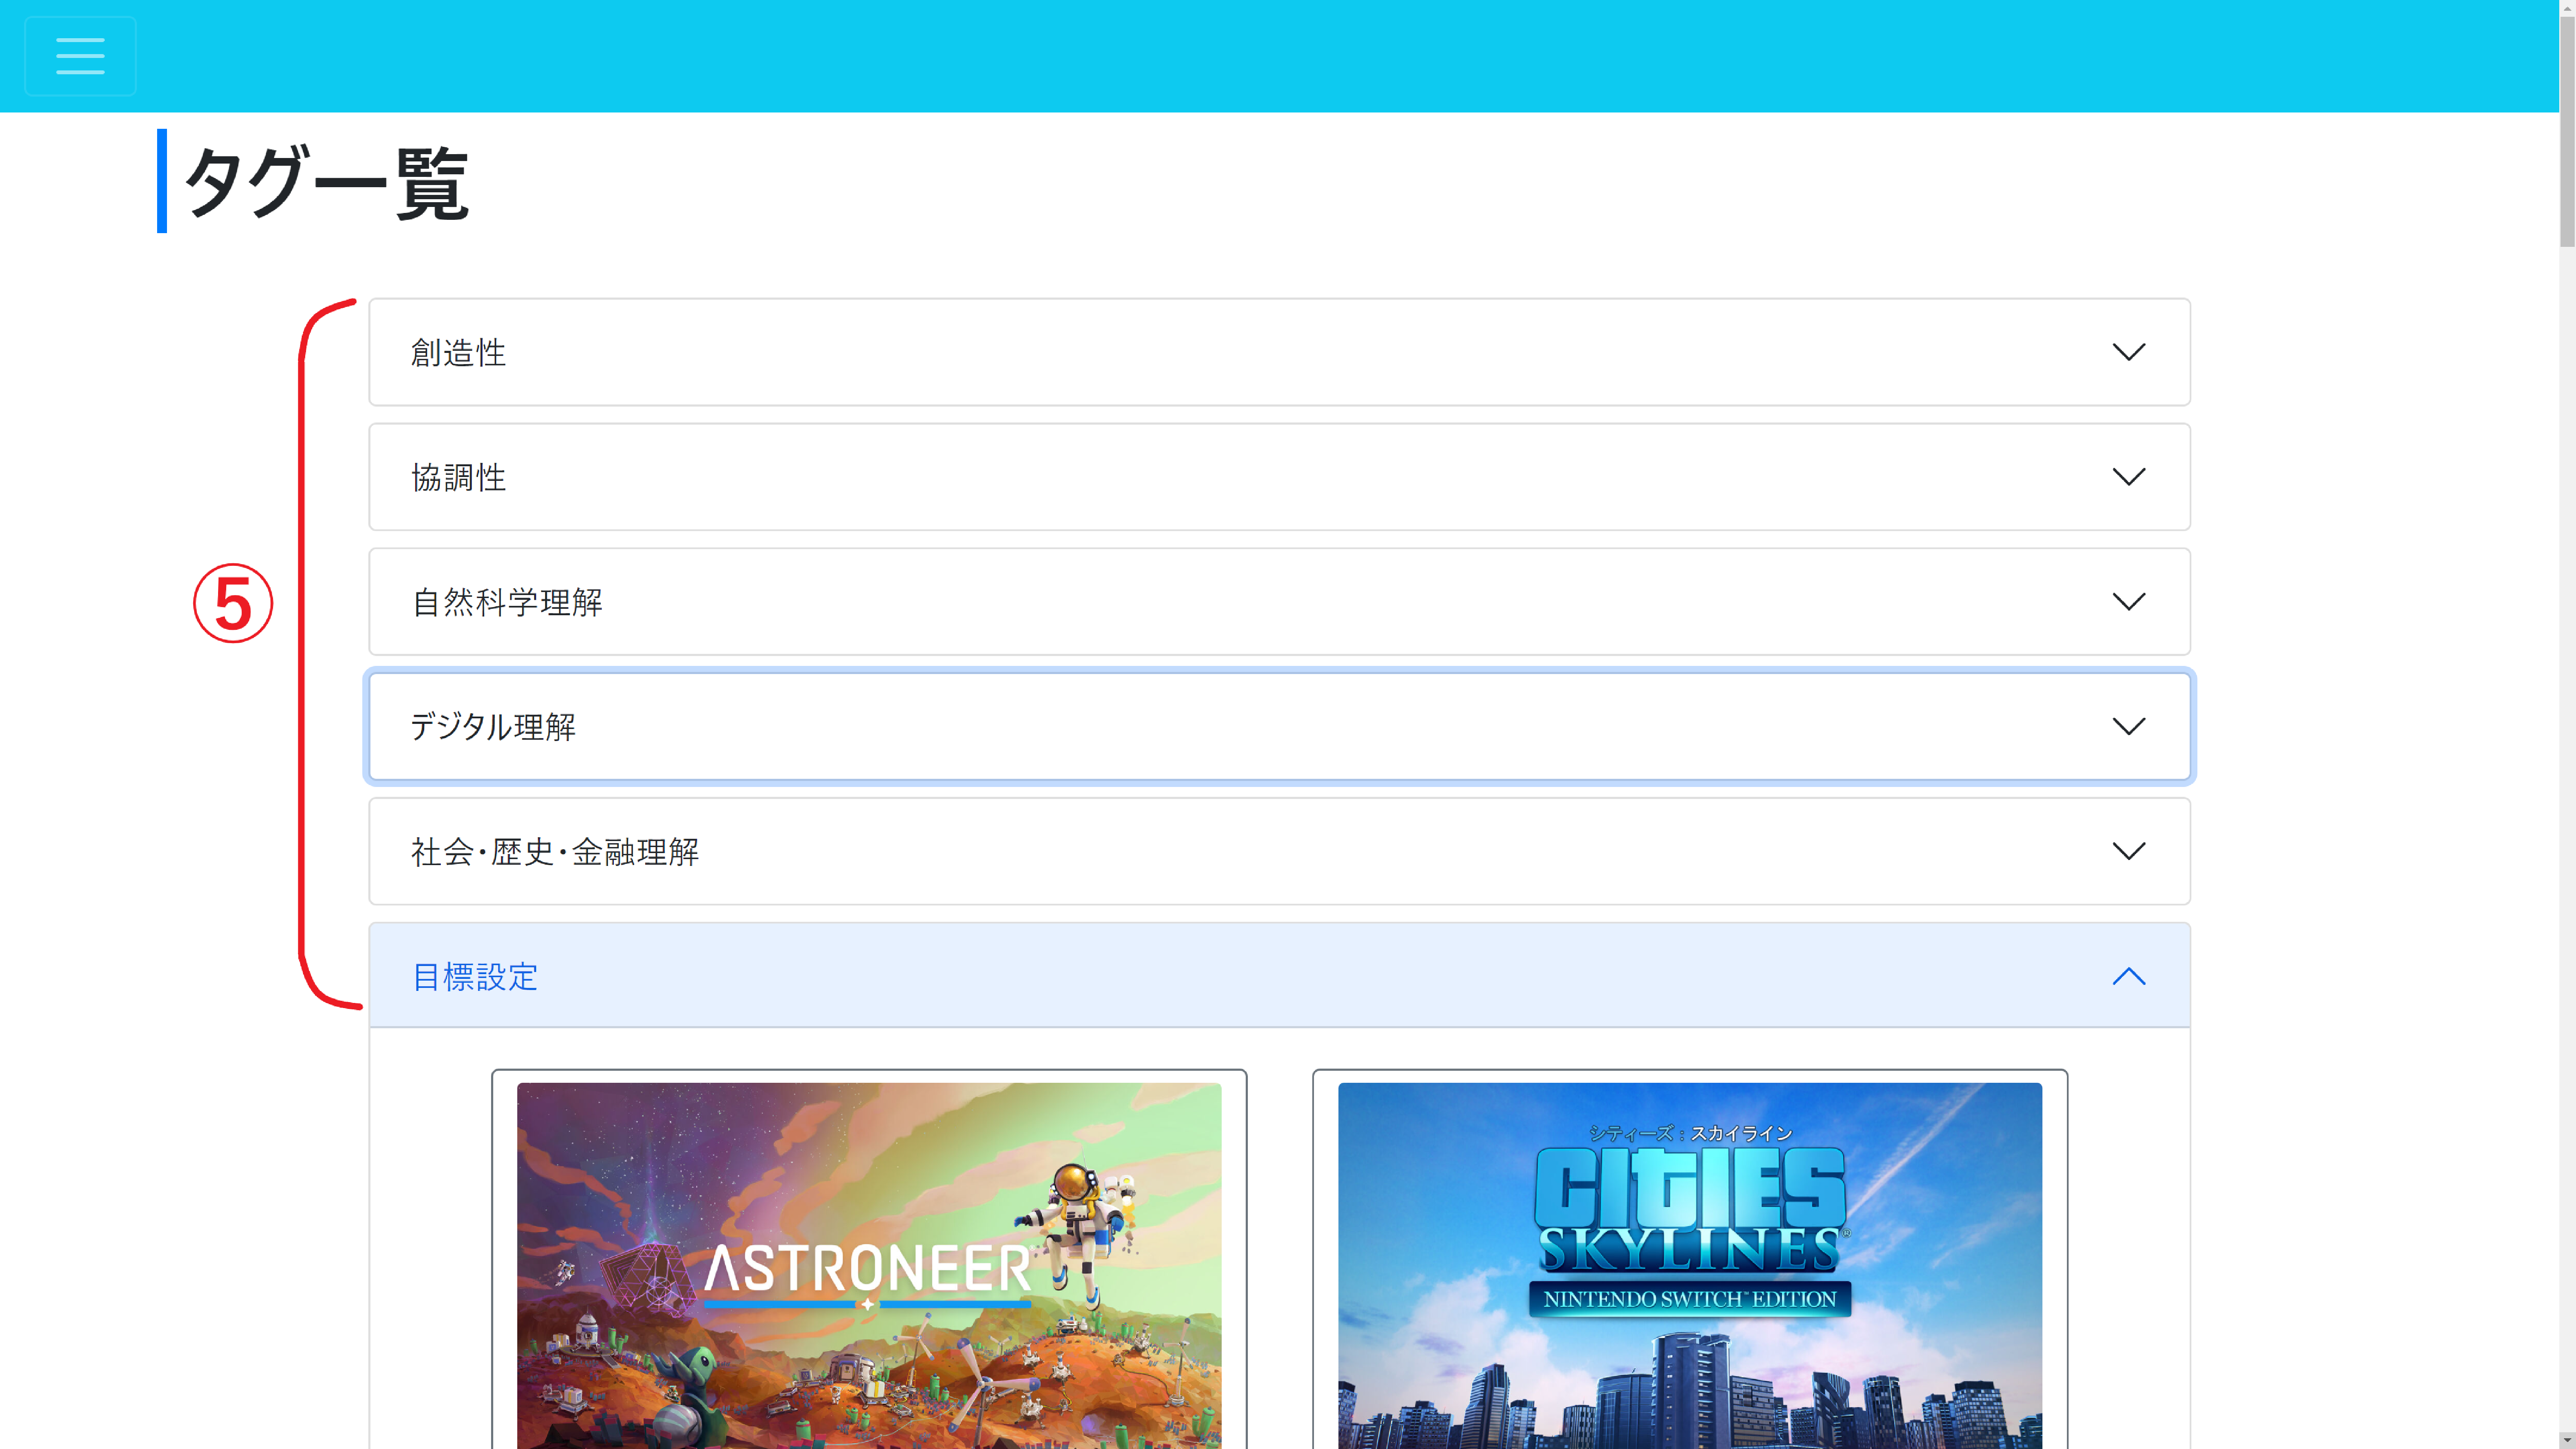
\includegraphics[keepaspectratio, scale=0.15]{PDF/tagpage.pdf}
\end{center}
 \caption{タグ一覧のページ}
 \label{fig:タグページ}
\end{figure}

教科一覧のページでは図\ref{fig:教科ページ}に示すように小中学校の教科を表示し,タグ一覧のページのようにアコーディオンメニューで関連するゲームとその記事へのリンクを設置した.

\begin{figure}[H]
\begin{center}
 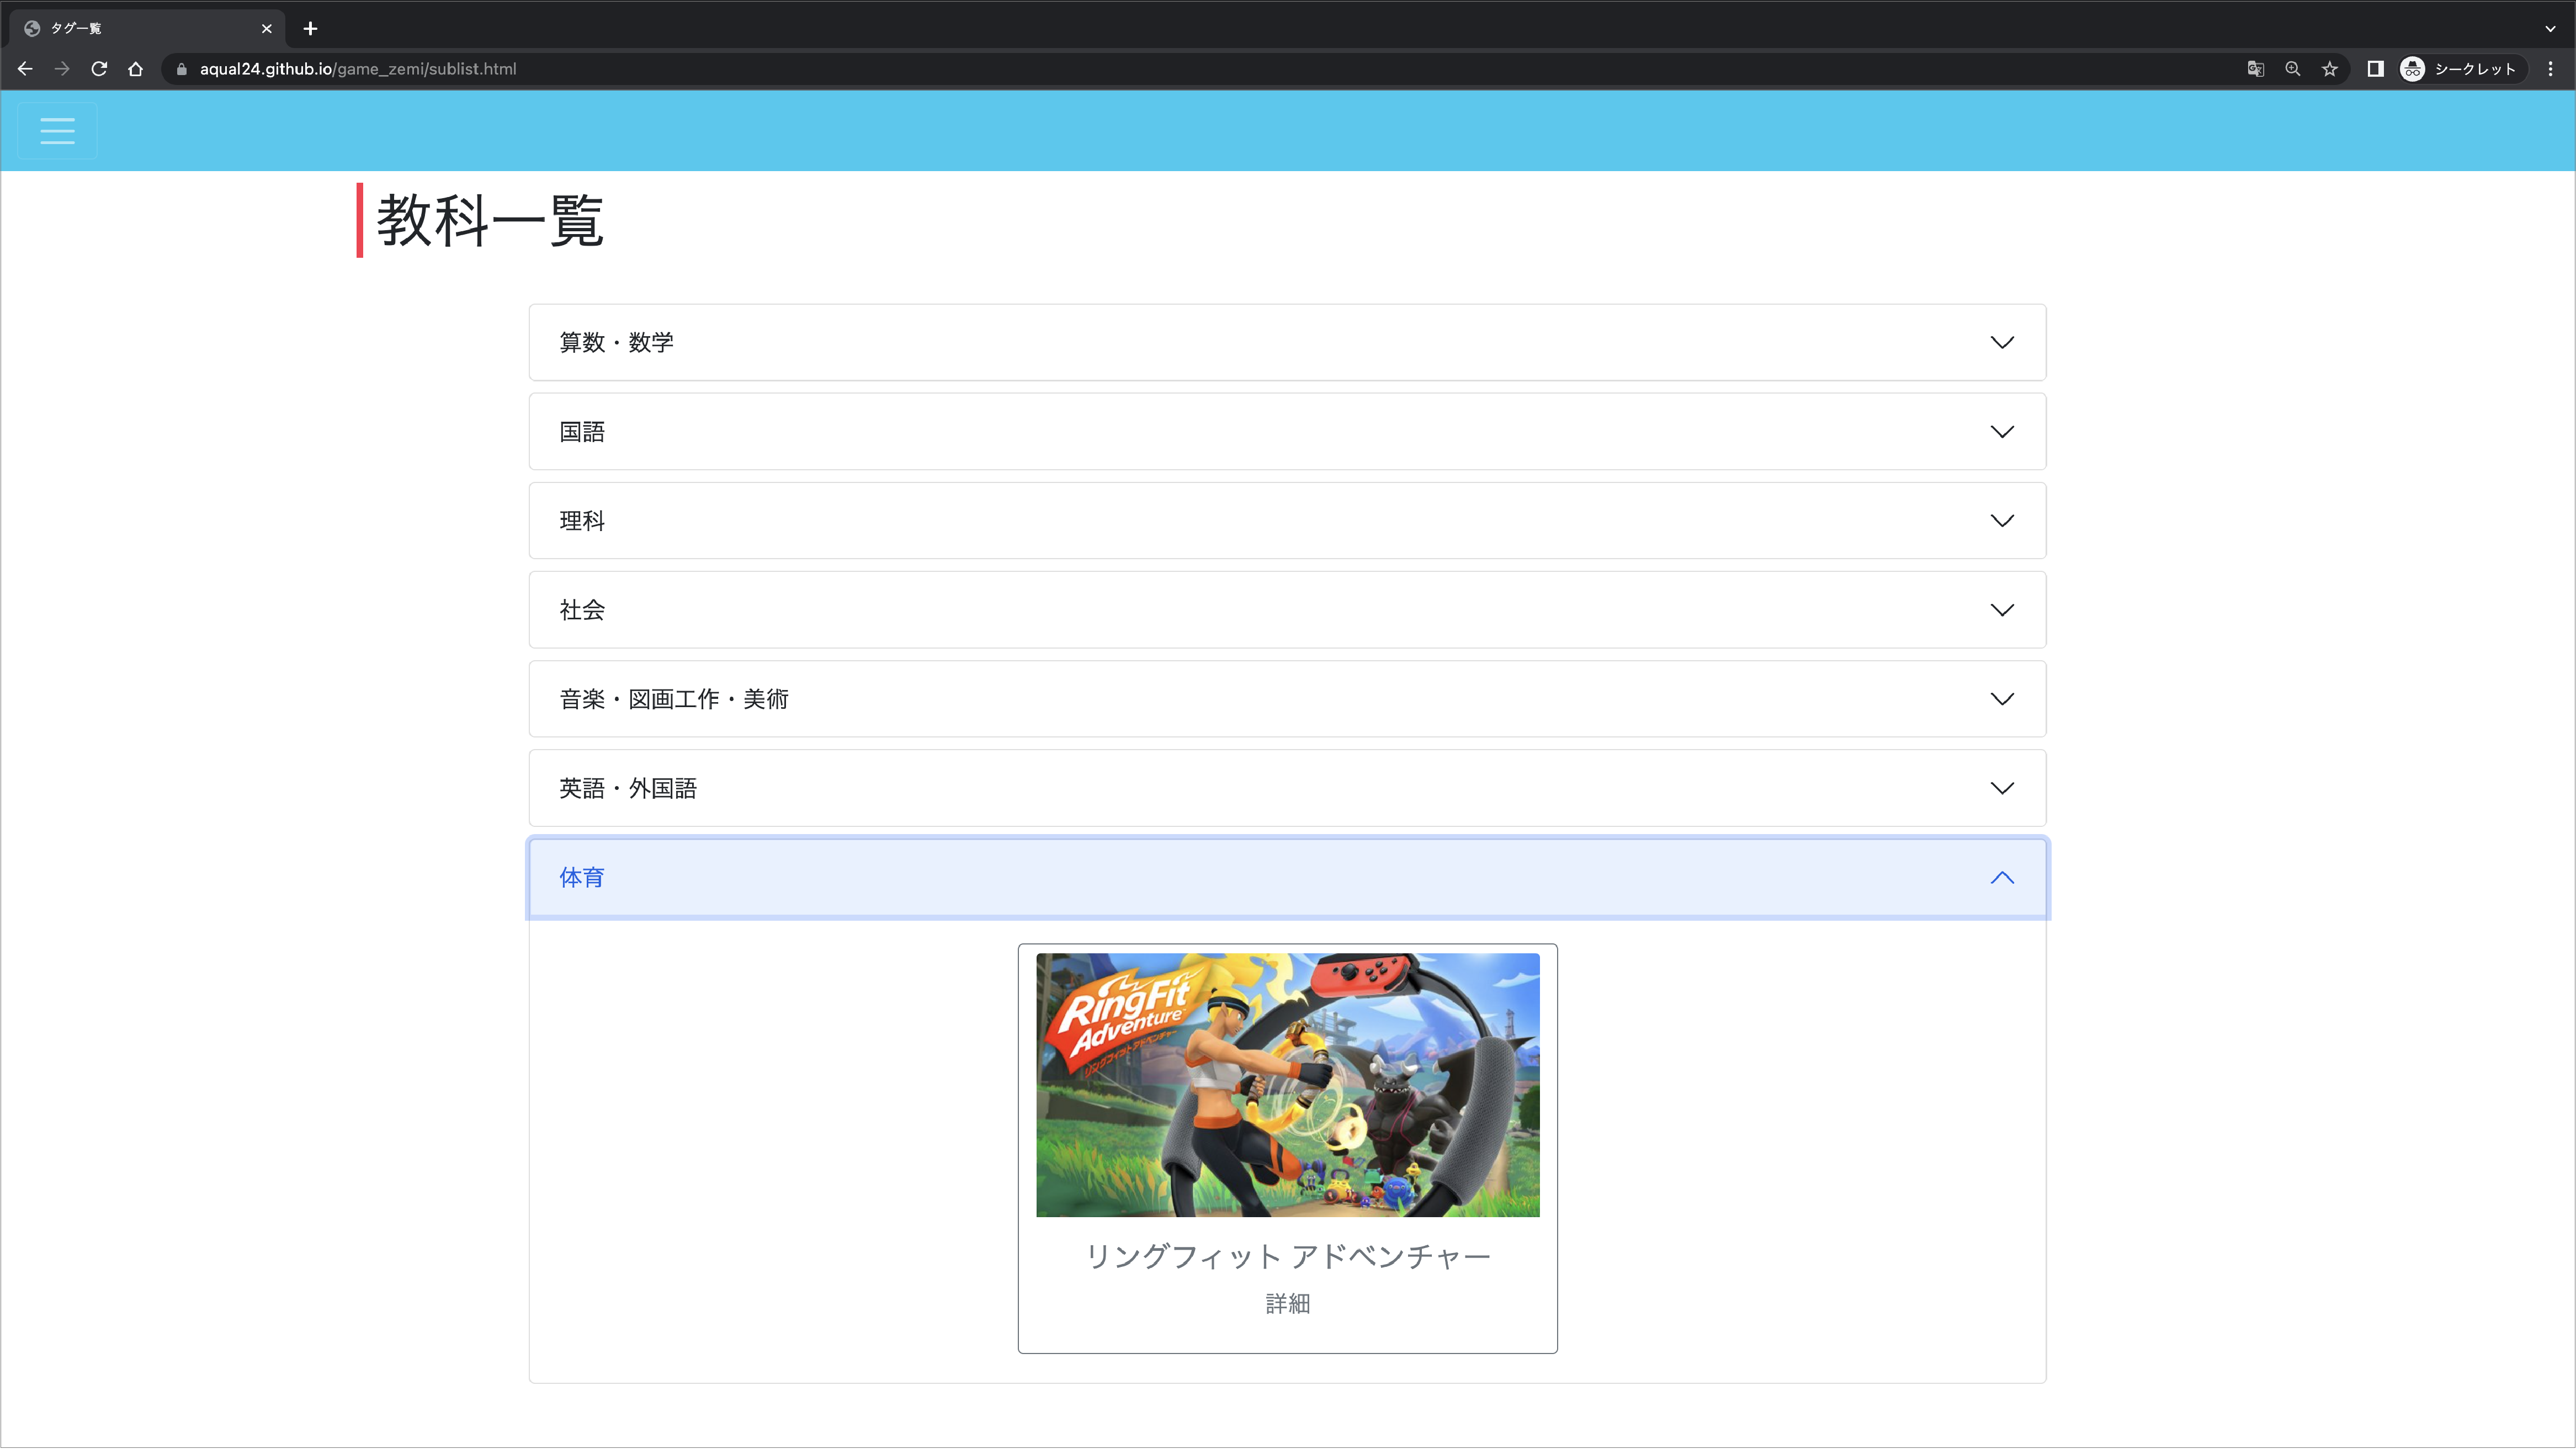
\includegraphics[keepaspectratio, scale=0.15]{PDF/subpage.pdf}
\end{center}
 \caption{教科一覧のページ}
 \label{fig:教科ページ}
\end{figure}

ゲーム一覧のページでは図\ref{fig:ゲーム一覧}に示すように「Nintendo Switch」とスマートフォンのアコーディオンメニューで対応するゲームとその記事のリンクを設置した.

\begin{figure}[H]
\begin{center}
 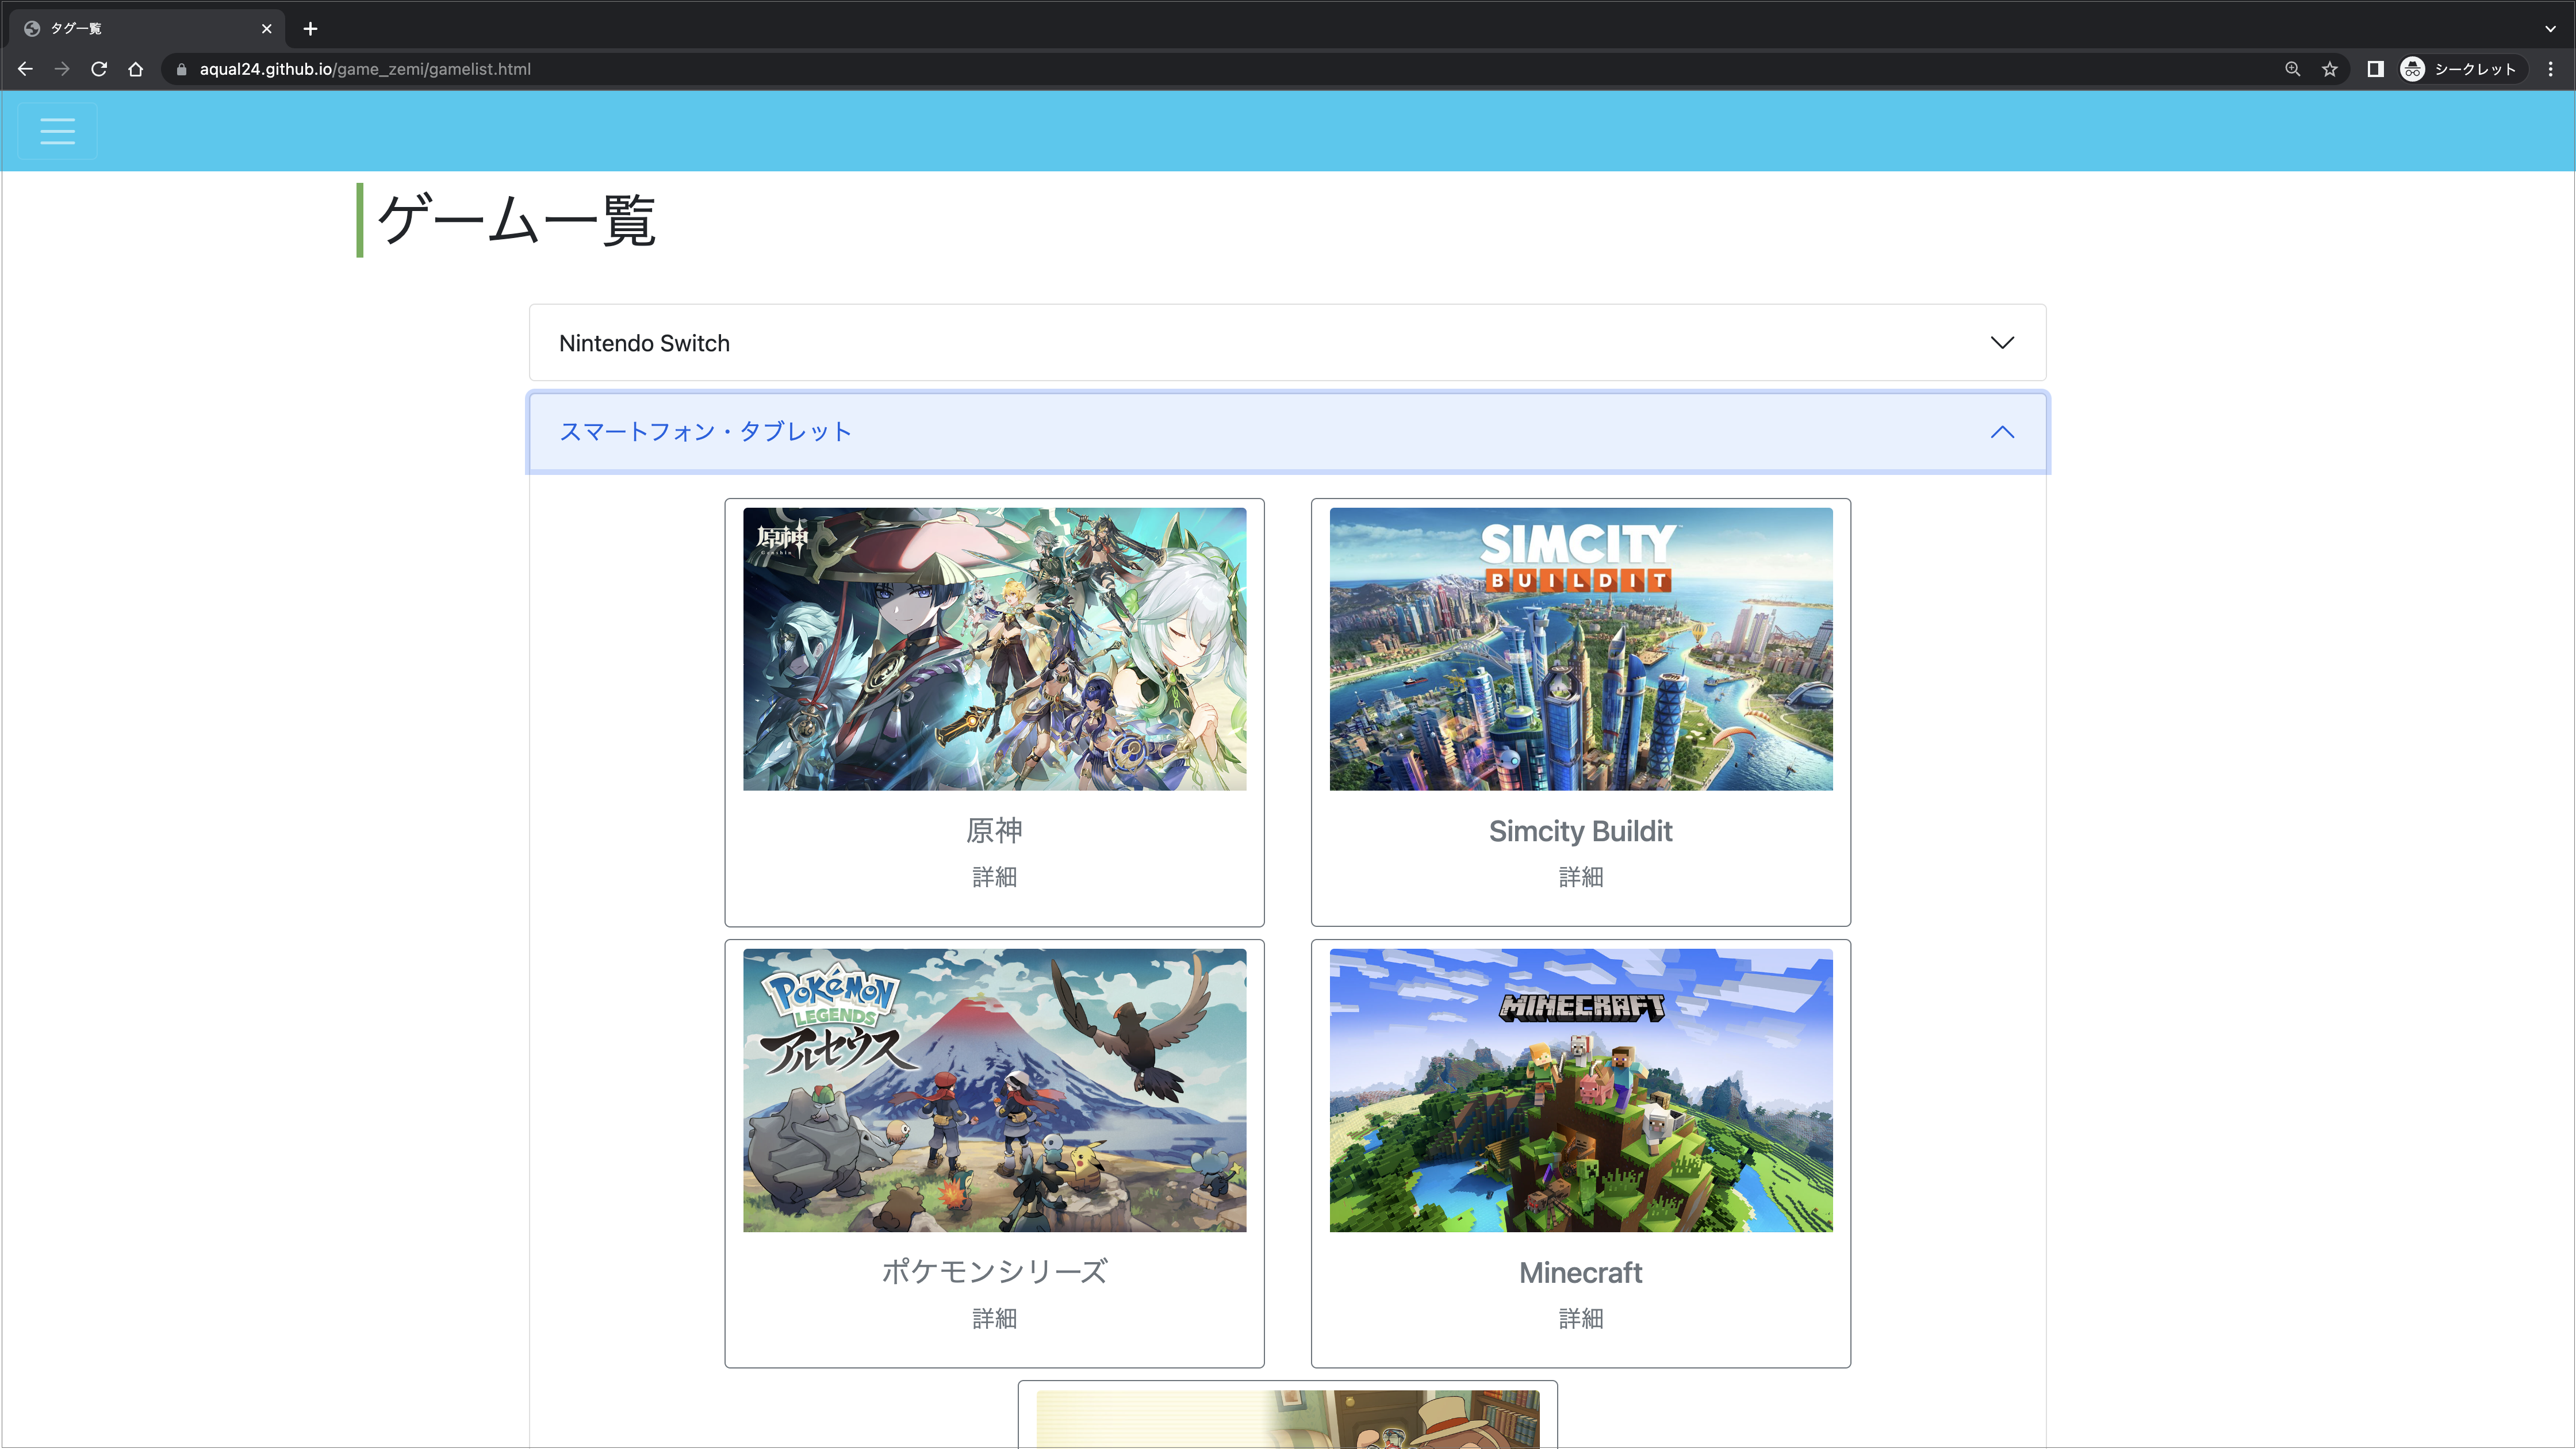
\includegraphics[keepaspectratio, scale=0.15]{PDF/gamepage.pdf}
\end{center}
 \caption{ゲーム一覧のページ}
 \label{fig:ゲーム一覧ページ}
\end{figure}

アンケートのページについてはず\ref{fig:アンケートページ}に示すように本研究の目的の簡易的な説明とアンケートの説明,対象者について記述し⑥にアンケートの回答ページへリンクするボタンを設置した.

\begin{figure}[H]
\begin{center}
 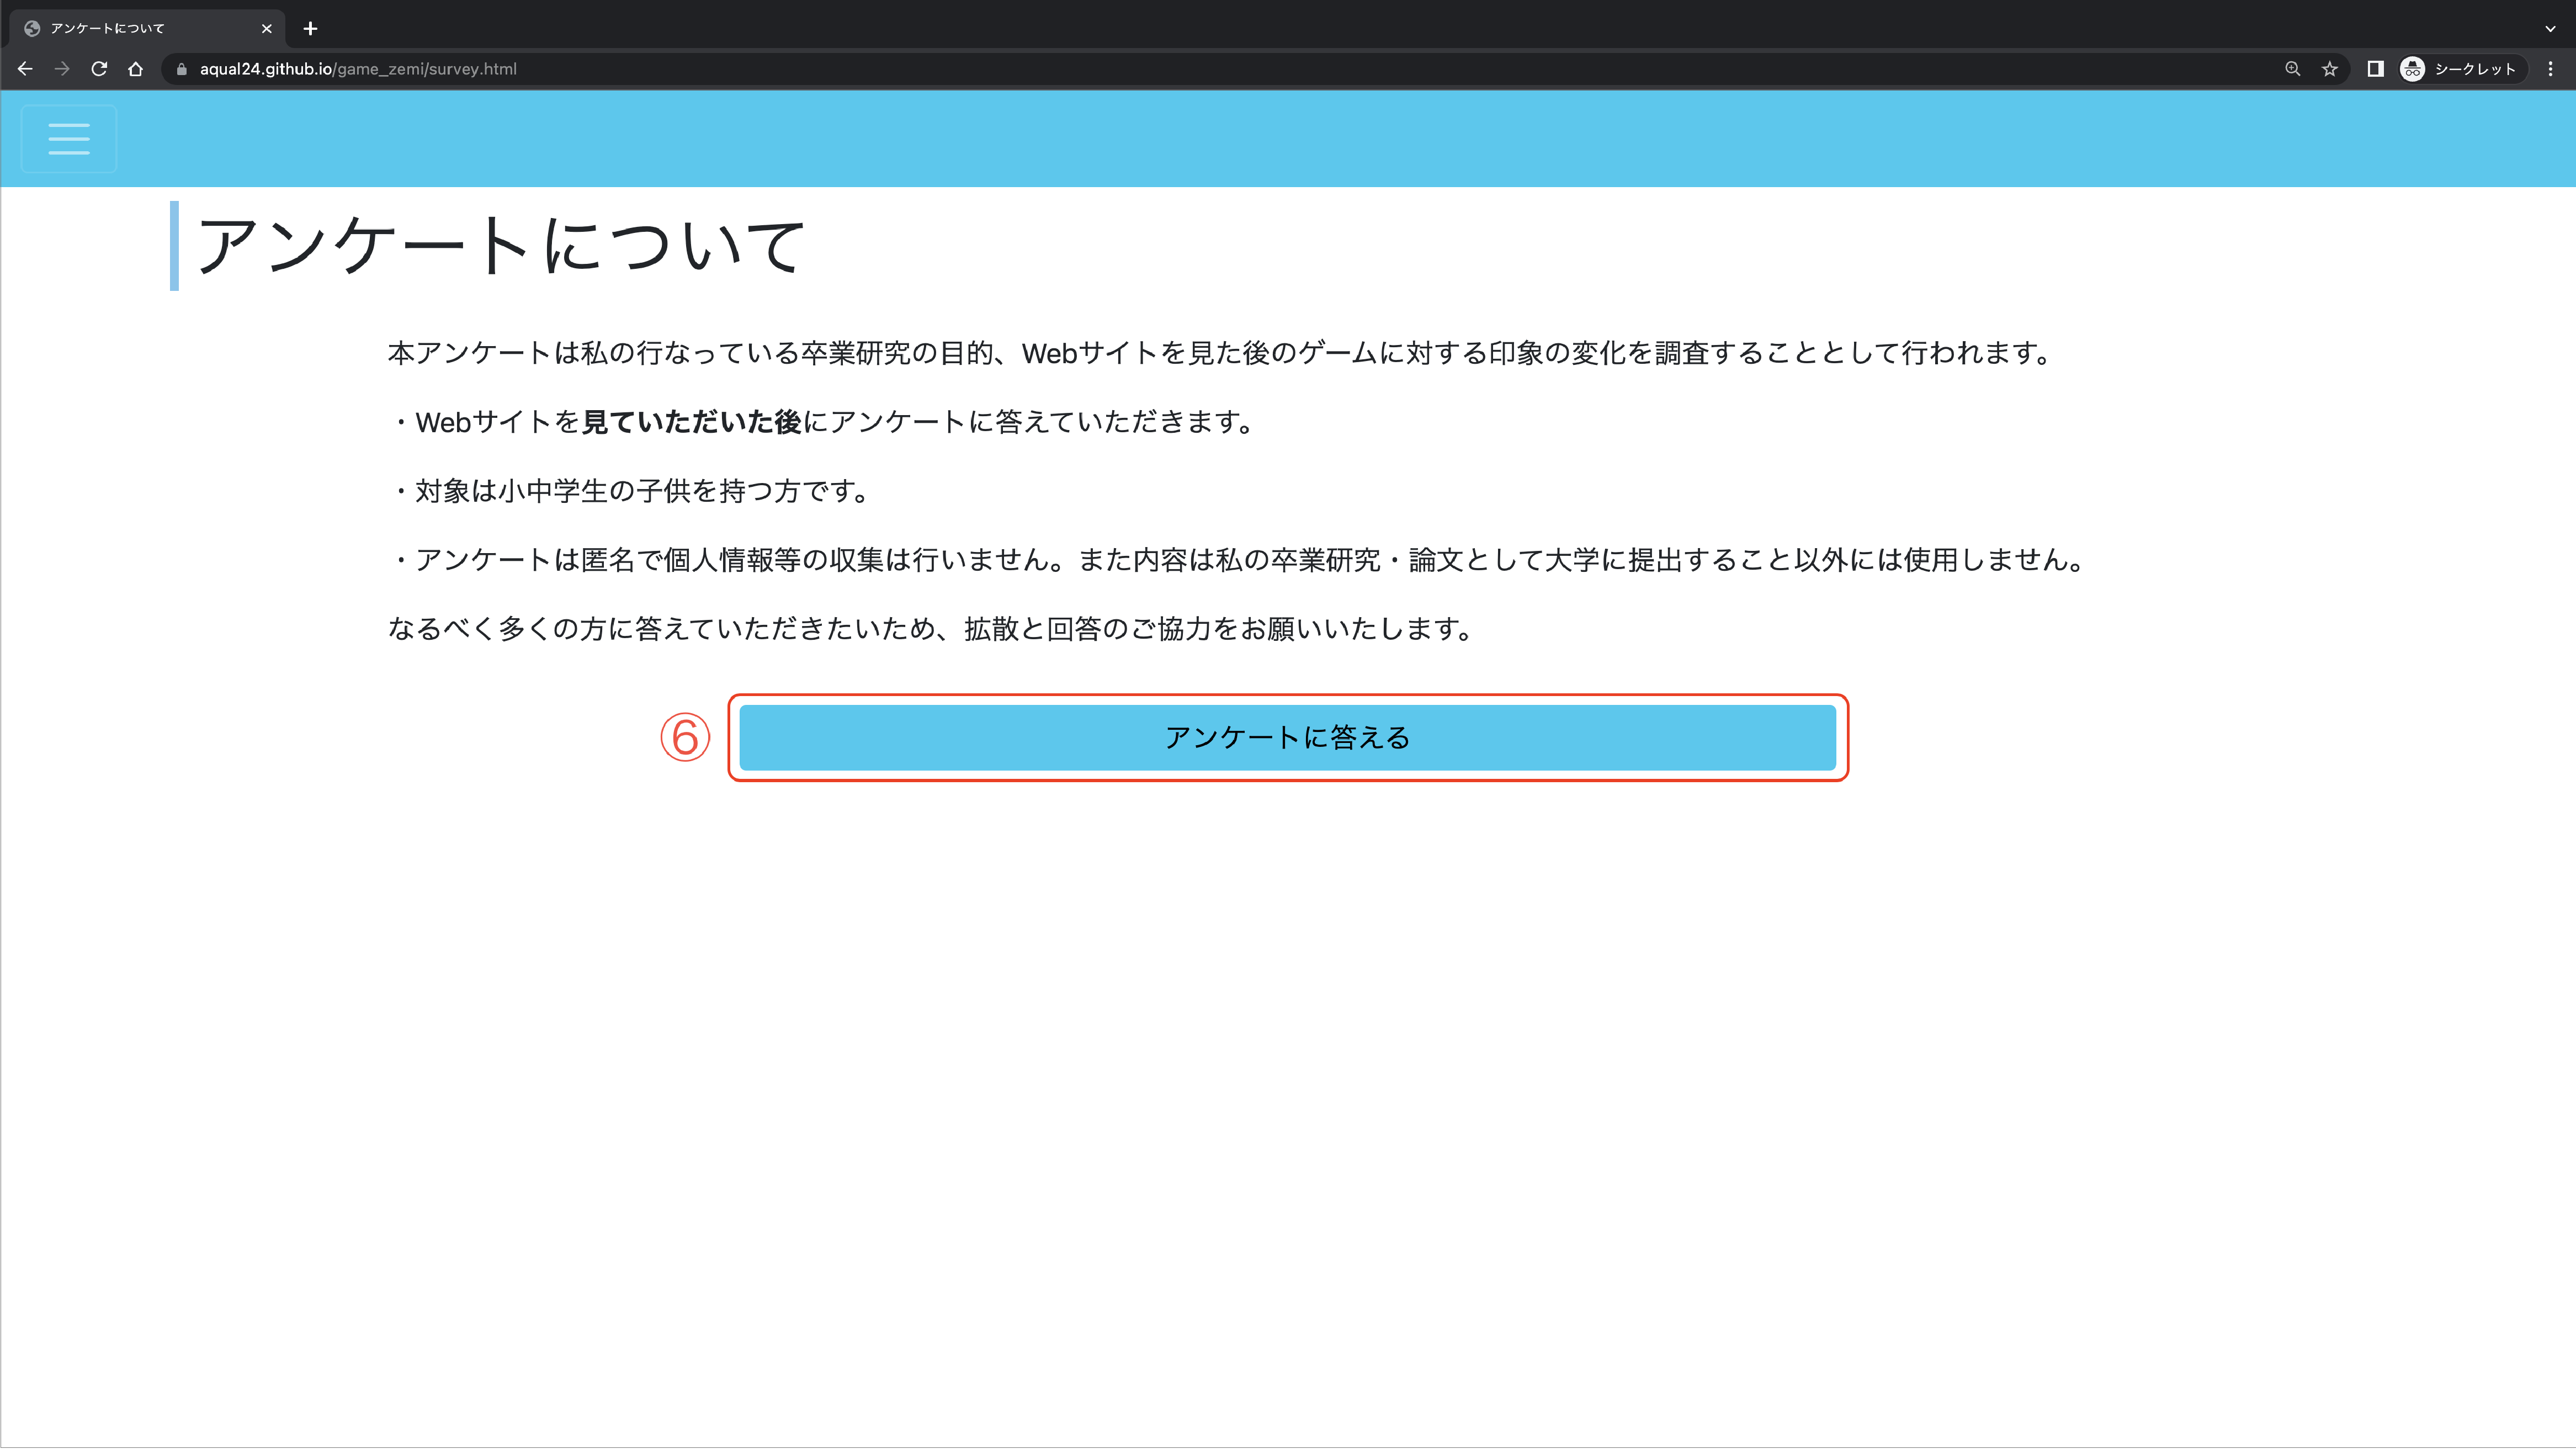
\includegraphics[keepaspectratio, scale=0.15]{PDF/anquepage.pdf}
\end{center}
 \caption{アンケートのページ}
 \label{fig:アンケートページ}
\end{figure}

ゲーム記事のページについては図\ref{fig:ゲームの記事}のようにゲームについての説明と教育観点からの説明を記述し最後部に公式サイトのリンクとゲームにタグ付された教育的なメリットと教科を表示した.

ゲーム記事についての詳細は\ref{ゲーム記事}に示す.

\begin{figure}[H]
\begin{center}
 \includegraphics[keepaspectratio, scale=0.6]{PDF/atsumoripage.pdf}
\end{center}
 \caption{ゲームの記事}
 \label{fig:ゲームの記事}
\end{figure}

\subsection{ゲームの種類}\label{ゲームの種類}
掲載したゲームは対象である小・中学生の年齢や傾向を加味し,Nintendo Switchのソフトとスマートフォンやタブレットでプレイできるゲームを12本に絞った.
また年齢に沿ったゲームの紹介を行う為,対象年齢を全年齢のもの9本と一部ゲーム内課金ができることやバトルシーンがあり12・15歳以上になっているもの3本を掲載した.
具体的なゲームの一覧は以下の図\ref{fig:ゲーム一覧}の通りである.

教育的なメリットについては図\ref{fig:ゲーム一覧}の右側上部のように「創造性」「思考力」「目標設定」「協調性」といったものの他に動植物や自然現象,科学についての「自然科学理解」,社会の仕組みや歴史,経済がどのようにして回っているかについての「社会・歴史。金融理解」,3D空間で移動や創作をすることで身につく「空間把握」,コンピュータやプログラムの仕組みについての「デジタル理解」の8本を扱った.
ゲームとメリットとの関連付けについては様々なコンテンツをプレイして身につくと思われるものを複数選択した.
またゲームと教科の関連付けについては選択した教育的なメリットと関係のある教科をそれぞれ選択した.
例としてNintendo Switchの「あつまれどうぶつの森」のタグ付けを図\ref{fig:ゲーム一覧}の右側に示す.

\vspace{1zh}
\begin{figure}[H]
\begin{center}
 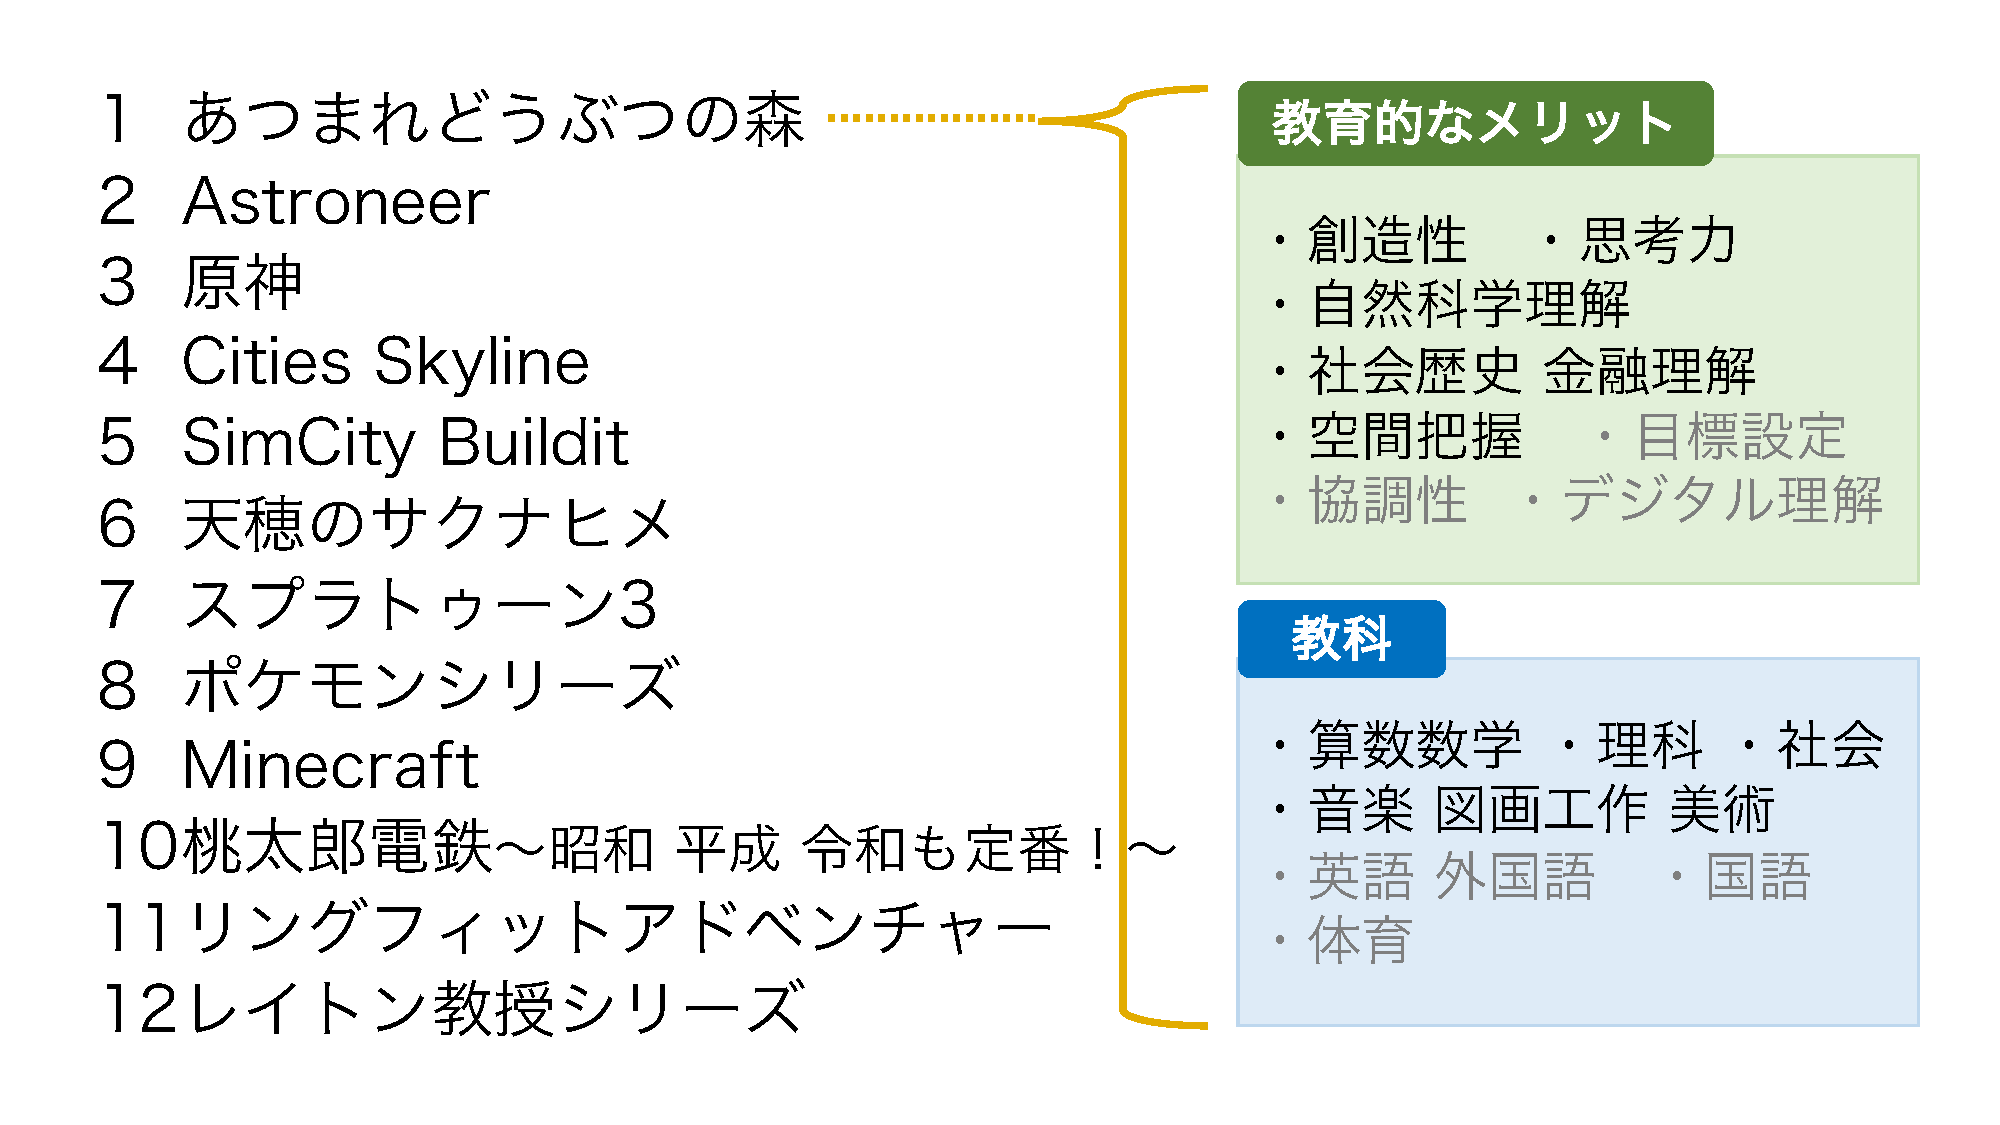
\includegraphics[keepaspectratio, scale=0.35]{PDF/games.pdf}
\end{center}
 \caption{ゲーム一覧とあつまれどうぶつの森のタグ付け例}
 \label{fig:ゲーム一覧}
\end{figure}

\newpage

\subsection{ゲーム記事}\label{ゲーム記事}
12本のゲームの記事のうちの一つである「あつまれどうぶつの森」について述べる.


\vspace{1zh}
\begin{figure}[H]
\begin{center}
 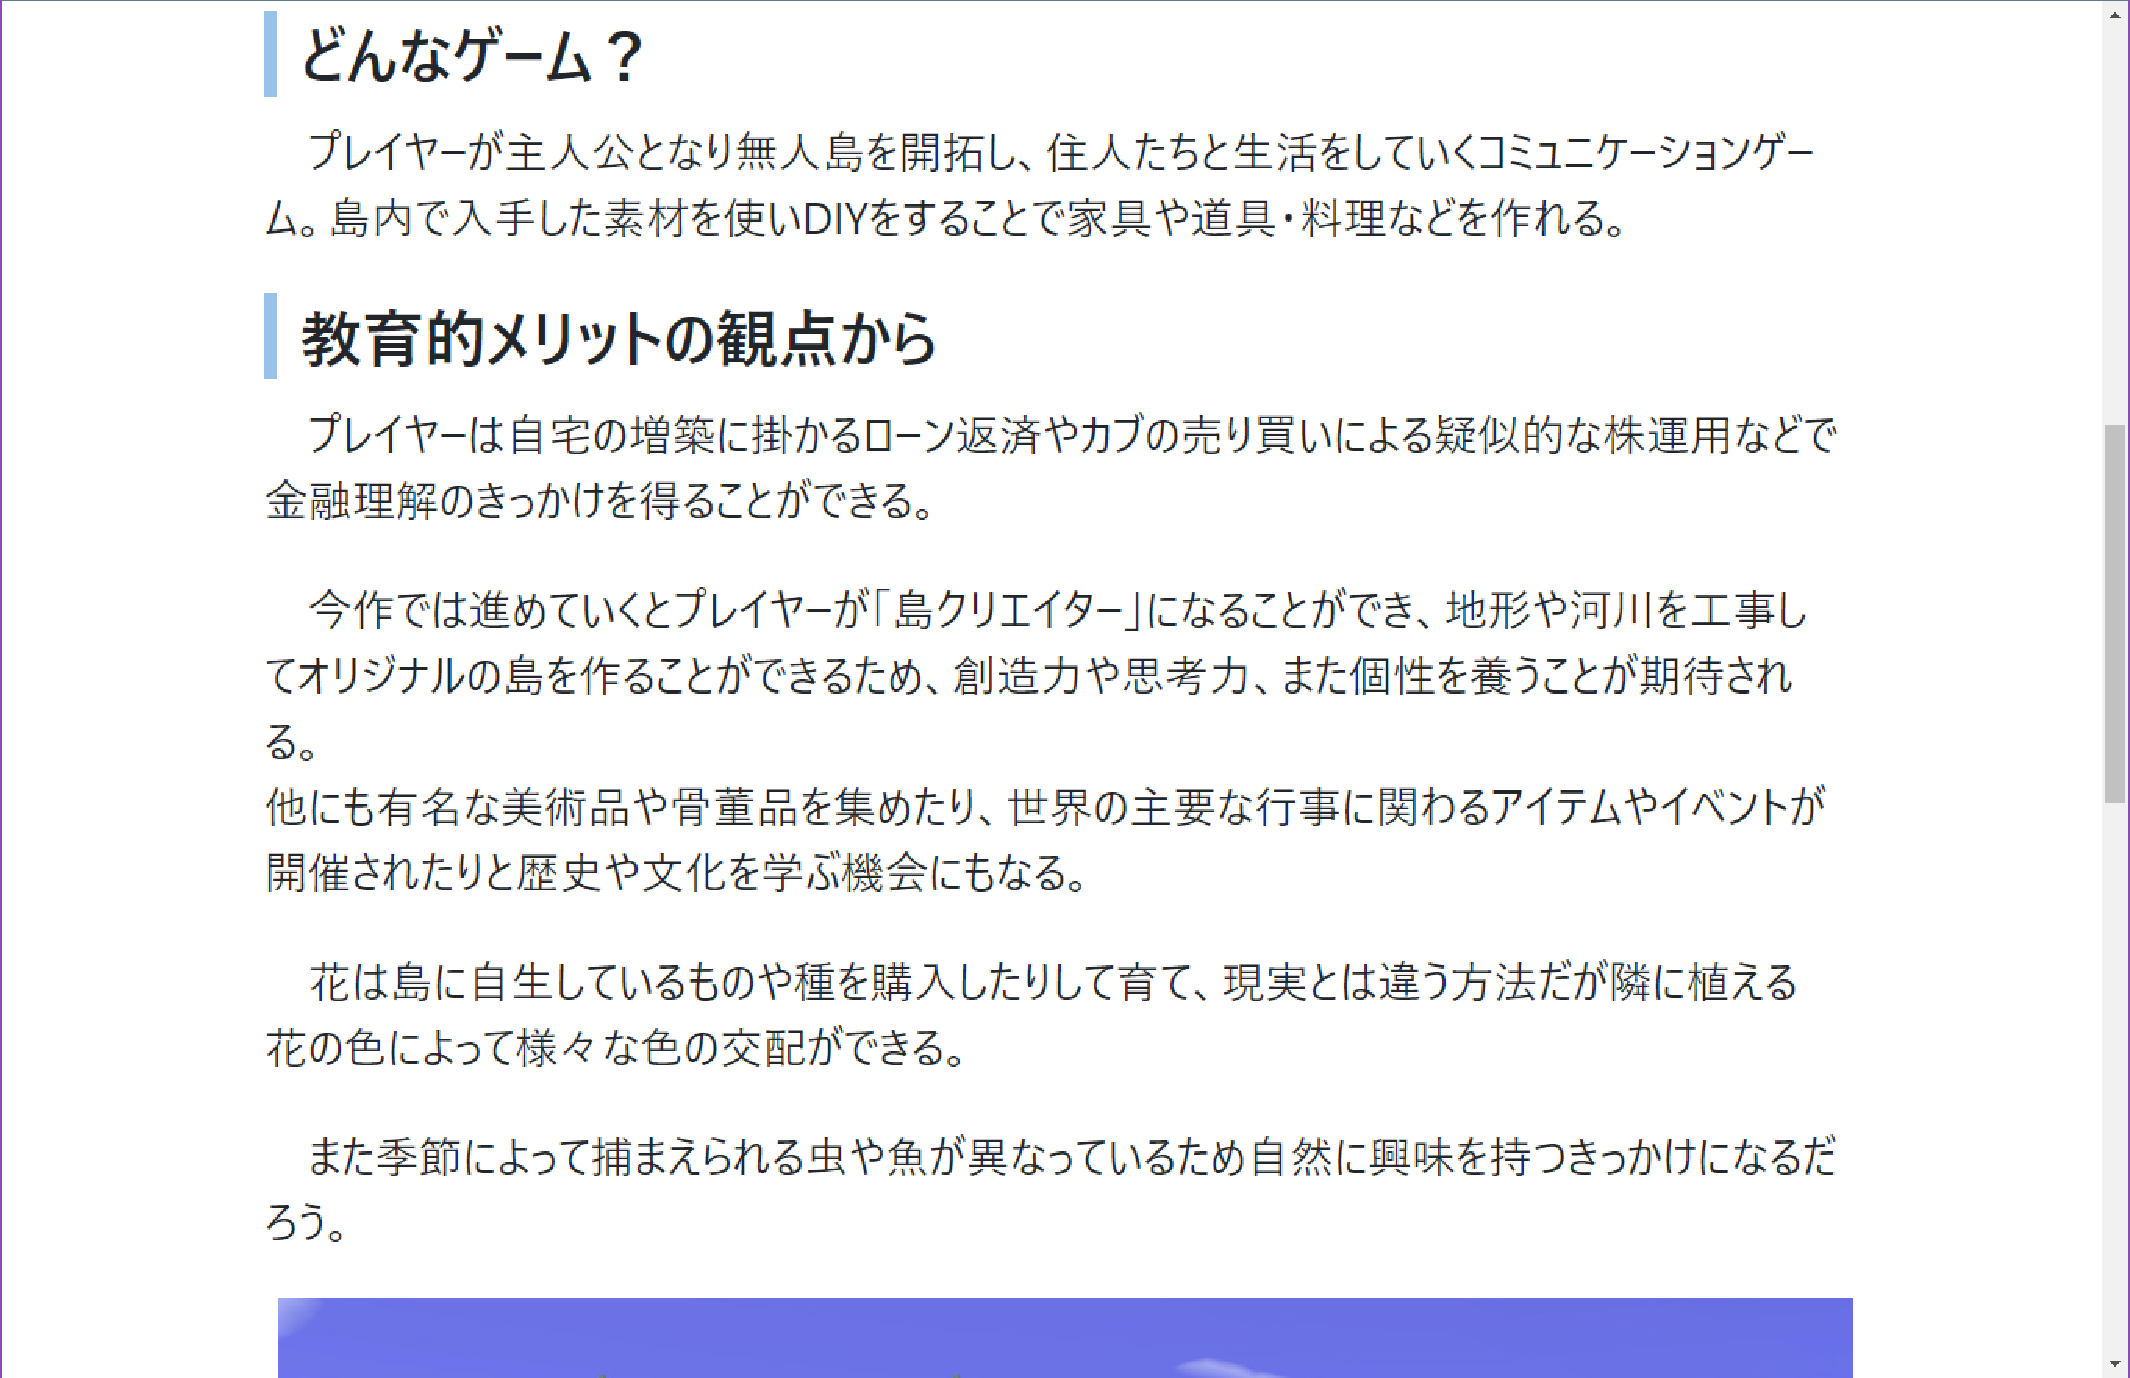
\includegraphics[keepaspectratio, scale=0.35]{PDF/あつ森1.pdf}
\end{center}
 \caption{あつまれどうぶつの森の記事}
 \label{fig:あつ森1}
\end{figure}



冒頭には図\ref{fig:あつ森1}の「どんなゲーム?」に示すようにゲームのジャンルであるコミュニケーションゲームということと大まかな内容や無人島という舞台,島内の素材を使い家具や道具などを作れるゲームということを簡易的に説明した.

次にゲームをプレイすることによって得られる学習効果を図\ref{fig:あつ森1}の「教育的メリットの観点から」に記した.
「あつまれどうぶつの森」は土地や河川を変形する,木や花を自由に植える,家具の配置,道具をクラフトすることができることから「創造力」と「空間把握」,「思考力」を設定した.
また季節によって取れるものが違う虫取りや魚釣りをすることで得られる図鑑や疑似的な花の交配ができることから「自然科学理解」を設定した.
さらに世界的に有名な実在する美術品の真贋を見極め収集することや家のローンの支払い,実際の株運用とは異なるものの疑似的な株の運用をする場面,世界の様々な文化や風習をイベントで学べる場面があるため「社会・歴史・金融理解」を設定した.
